% !TeX root = ../SigSysBoxen.tex

	\chapter{Motivation, Wiederholung und Überblick}
\begin{tbox}
	a
\end{tbox}

\begin{abox}
	\underline{U}_1 &= U_1 \angle \varphi_1 = \frac{30}{\sqrt{2}} \angle \frac{\pi}{3}\\
	\underline{Z}_R &= R = 1000\\
	\underline{Z}_C &= \frac{1}{j \omega C} = \frac{1}{sC} = \frac{1000}{s}
\end{abox}

\begin{abox}
	H(s) := \frac{\underline{U}_2}{\underline{U}_1} = \frac{\underline{Z}_C}{\underline{Z}_R + \underline{Z}_C} = \frac{\frac{1}{sC}}{R + \frac{1}{sC}} = \frac{1}{1 + sRC} = \frac{1}{1 + s}
\end{abox}

\begin{abox}
	\left|H(j\omega)\right| &= \left|\frac{1}{1 + j\omega RC}\right| = \frac{1}{\left|1 + j\omega RC\right|} = \frac{1}{\sqrt{1^2 + (\omega RC)^2}} = \frac{1}{\sqrt{1 + \omega^2}}\\
	\sphericalangle H(j\omega) &= \sphericalangle \frac{1}{1 + j\omega RC} = \sphericalangle \frac{1 - j \omega RC}{1 + (\omega RC)^2} = \arctan\left(\frac{\frac{-\omega RC}{1 + (\omega RC)^2}}{\frac{1}{1 + (\omega RC)^2}}\right)\\
	&= \arctan(\omega RC) = -\arctan(\omega)\\
	\underline{U}_2 &= H(s) \cdot \underline{U}_1 = \left|H(j\omega)\right| \cdot \left|\underline{U}_1\right| \angle\varphi_1 \sphericalangle H(j\omega)\\
	&= \frac{1}{\sqrt{1 + \omega^2}} \cdot \left|\underline{U}_1\right| \angle (\frac{\pi}{3} - \arctan(\omega))
\end{abox}

\begin{abox}
	a) \quad\underline{U}_2 &= \frac{1}{\sqrt{1 + (2\pi \cdot 0,5)^2}} \cdot 21.2 \angle \frac{\pi}{3} - \arctan(2\pi \cdot 0,5) \approx 6,43\angle -0,21\\
	&\Rightarrow u_2(t) = 6,43 \cdot\sqrt{2} \cdot \sin(2\pi \cdot 0,5 \cdot t - 0,21) \approx \SI{9,09}{\volt} \cdot \sin(\pi t - 0,21)\\
	b) \quad\underline{U}_2 &\approx 0,67\angle -0,49 \Rightarrow u_2(t) \approx \SI{0,95}{\volt} \cdot \sin(10\pi t - 0,49)\\
	c) \quad\underline{U}_2 &\approx 0,0067\angle -0,523 \Rightarrow u_2(t) \approx \SI{9,55}{\milli\volt} \cdot \sin(100\pi t - 0,523)
\end{abox}

\begin{abox}
	&\text{Für}\quad x(t) = \SI{30}{\volt}\sin(\pi t + \pi / 3)\quad \text{ist}\quad \mathcal{H}\{x(t)\} = \SI{9,09}{\volt}\sin(\pi t - 0,21)\\
	&\text{Für}\quad y(t) = \SI{30}{\volt}\sin(10\pi t + \pi / 3)\quad \text{ist}\quad \mathcal{H}\{y(t)\} = \SI{0,95}{\volt}\sin(10\pi t - 0,49)
\end{abox}

\begin{tbox}
	\begin{align*}
	u_1(t) = \SI{15}{\volt}\sin(\pi t + \pi/3) + \SI{60}{\volt}\sin(10\pi t + \pi/3) = 0,5x(t) + 2y(t)
	\end{align*}
	und damit $a = 0,5, b=2$ und
	\begin{align*}
	u_2(t):= \mathcal{H}\{u_1(t)\} = \mathcal{H}\{0,5x(t) + 2y(t)\} \overset{??}{=}
	\end{align*}
\end{tbox}

\begin{abox}
	&\mathcal{H}\{ax(t) + by(t) + cz(t)\} = \mathcal{H}\{ax(t) + 1 \cdot (by(t) + cz(t)\}\\
	&\overset{(??)}{=} a\mathcal{H}\{x(t)\} + 1 \cdot \mathcal{H}\{by(t) + cz(t)\} \overset{(??)}{=} a\mathcal{H}\{x(t)\} + b\mathcal{H}\{y(t)\} + c\mathcal{H}\{z(t)\}
\end{abox}

\begin{abox}
	x[-\infty],\dots,x[-3],x[-2],x[-1],x[0],x[1],x[2],x[3],\dots,x[\infty]
\end{abox}

\begin{tbox}
	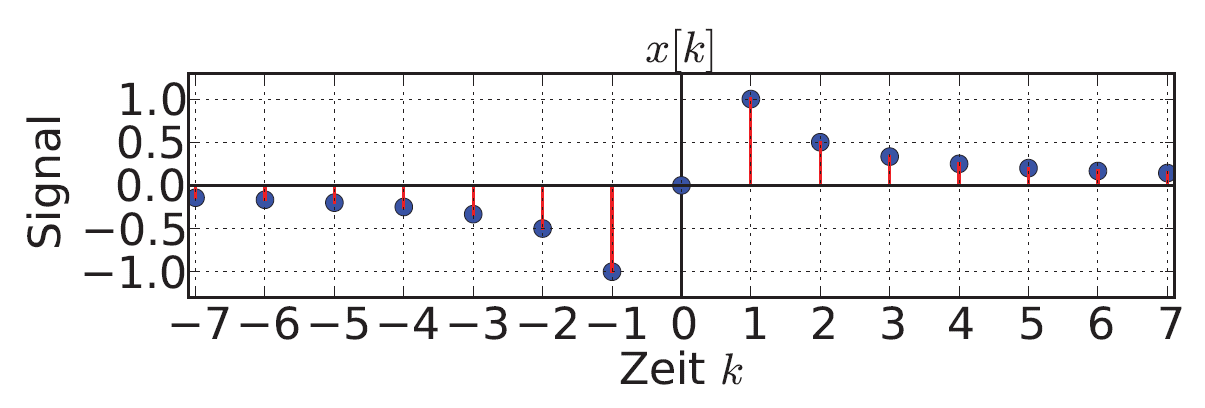
\includegraphics[width=\textwidth]{Box9}
\end{tbox}

\begin{tbox}
	\begin{itemize}
		\item $x[-k]$ die \underline{Spiegelung} von $x[k]$ an der Signalpegel-Achse
		\item  $x[k + k_0]$ die \underline{Verschiebung von $x[k]$ um $k_0$ nach links}
		\item  $x[k - k_0]$ die \underline{Verschiebung von $x[k]$ um $k_0$ nach rechts}
	\end{itemize}
\end{tbox}

\chapter{Diskrete Signale}
\setcounter{BoxCounter}{10}
\begin{tbox}
\end{tbox}

\begin{tbox}
	\begin{alignat*}{2}
	&(b) \quad x[-k] &&= \begin{cases}
	-\frac1k,\quad k \ne 0 \\
	0,\quad k = 0
	\end{cases}
	\\
	&(c)\quad  x[k+k_0] = x[k+3] &&= \begin{cases}
	\frac{1}{k+3}, \quad k \ne -3 \\
	0, \quad k = -3
	\end{cases}\\
	&(d)\quad  x[k-k_0] = x[k-3] &&= \begin{cases}
	\frac{1}{k-3}, \quad k \ne 3 \\
	0, \quad k = 3
	\end{cases}
	\end{alignat*}
\end{tbox}

\begin{abox}
	x[k_0 - k] &= x[-(k - k_0)]\\
	&= x[(-k) + k_0]
\end{abox}

\begin{abox}
	\text{mit} \quad x[k_0 -k] = x[3 - k] = \begin{cases}
		\frac{1}{3-k}, \quad k \ne 3\\0 , \quad k = 3
	\end{cases}
\end{abox}

\begin{tbox}
	\begin{itemize}
		\item $x[k]$ heißt \underline{gerades Signal}, falls $x[k] = x[-k]$ $\forall k \in \mathbb{Z}$ gilt.
		\item $x[k]$ heißt \underline{ungerades Signal}, falls $x[k] = -x[-k]$ $\forall k \in \mathbb{Z}$ gilt.
	\end{itemize}
\end{tbox}

\begin{abox}
	x[-k] = \begin{cases}
		\frac{1}{-k}, \quad k \ne 0\\
		0, \quad k = 0
	\end{cases} = \begin{cases}
		-\frac1k, \quad k \ne 0 \\ 
		0, \quad k = 0 
	\end{cases}  = -x [k] 
\end{abox}

\begin{abox}
	y[-k] = \begin{cases}
		\frac{1}{(-k)^2}, \quad k \ne 0\\
		0, \quad k = 0
	\end{cases} = \begin{cases}
		-\frac{1}{k^2}, \quad k \ne 0 \\
		0, \quad k = 0 
	\end{cases}  = y [k] 
\end{abox}

\begin{tbox}
	\begin{itemize}
		\item  $x[k]$ heißt \underline{kausales Signal}, falls gilt: $x[k] = 0$ $\forall k < 0$
		\item $x[k]$ heißt \underline{nicht-kausales Signal}, falls gilt $\exists k < 0 : x[k] \ne 0$
		\item $x[k]$ heißt \underline{anti-kausales Signal}, falls $x[-k-1]$ kausal ist, d.h. falls gilt: $x[k] = 0$ $\forall k \leqslant 0$
	\end{itemize}
\end{tbox}

\begin{tbox}
	\begin{itemize}
		\item $x[k]$ ist nicht-kausal
		\item $u[k]$ ist kausal
		\item $v[k]$ ist anti-kausal
	\end{itemize}
\end{tbox}

\begin{abox}
	\delta[k] := \begin{cases}
		1, \quad k = 0\\ 0, \quad k \ne 0
	\end{cases}
\end{abox}

\begin{abox}
	\epsilon[k] := \begin{cases}
		1, \quad k \ge 0\\ 0, \quad k < 0
	\end{cases}
\end{abox}

\begin{dbox}[width=0.45\textwidth]
	\begin{align*}
	\delta[k-k_0] = \begin{cases}
	1, \quad k = k_0\\ 0, \quad k \ne k_0
	\end{cases}
	\\ \text{bzw.} \\
	\delta[k+k_0] = \begin{cases}
	1, \quad k \ne -k_0\\ 0, \quad k = -k_0
	\end{cases}
	\end{align*}
\end{dbox}

\begin{dbox}[width=0.45\textwidth]
	\begin{align*}
	x[k]\cdot \delta[k-i] &= \begin{cases}
	x[i], \quad k = i \\ 0, \quad k \ne i
	\end{cases}\\
	&= x[i] \cdot \delta[k-i] \numbereq \\
	\text{Siebeigenschaft}
	\end{align*}
\end{dbox}


\begin{abox}
	x[k] = \sum_{i= -\infty}^{\infty} x[i]\cdot\delta[k-i] \quad \text{für alle} \quad k \in \mathbb{Z}
\end{abox}

\begin{abox}
	x[k] = \sum_{i= -K}^{K} x[i]\cdot\delta[k-i]
\end{abox}

\begin{abox}
	u[k] &= \delta[k + 2] + \delta[k + 1] + \delta[k] + \delta[k - 1]\\
	v[k] &= 2\cdot\delta[k + 3] + \delta[k + 1] - \delta[k - 1] - 2\cdot\delta[k - 3]
\end{abox}

\begin{abox}
	sgn[k]:= \epsilon[k] - \epsilon[-k] = \begin{cases}
		1, \quad k > 0\\0, \quad k=0\\-1, \quad k<0
	\end{cases}
\end{abox}

\begin{abox}
	\KW [k] := \epsilon[k] + \epsilon[-k-1] = 1 \text{ für alle } k \in \mathbb{Z}
\end{abox}

\begin{abox}
	rect_{k_{1}, k_{2}}[k] := \epsilon[k-k1] - \epsilon[k-k_2-1] = \begin{cases}
		1, \quad k_1\leqslant k \leqslant k_2
	\end{cases}
\end{abox}

\begin{abox}
	x[k] = q^k \cdot \epsilon[k]
\end{abox}

\begin{abox}
	x[k]: 0, ..., 0, x[0] = 1, x[1]=-0.7,x[2]=0.49,x[3]= 0.343, ...
\end{abox}

\begin{abox}
	x[k]: 0, ..., 0, x[0] = 1, x[1]=-0.8,x[2]=0.64,x[3]= -0.512, ...
\end{abox}

\begin{abox}
	x[k] + y[k] &: x[-\infty] + y[-\infty]  ..., x[0] + y[0], x[1] + y[1], ... , x[\infty] + y[\infty]\\
	x[k] \cdot y[k] &: x[-\infty] \cdot y[-\infty]  ..., x[0] \cdot y[0], x[1] \cdot y[1], ... , x[\infty] \cdot y[\infty]\\
	c \cdot x[k] &: c \cdot x[-\infty]  ..., c \cdot x[0], c \cdot x[1], ... , c \cdot x[\infty]\\
\end{abox}

\begin{abox}
	S_{k_1,k_2} := \{\overrightarrow{x} \in S|x[k] = 0 \text{ } \forall k < k_1 \text{ oder } k>k_2\}
\end{abox}

\begin{tbox}
	\begin{alignat*}{6}
	\overrightarrow{x} &&= (0 \quad & 3 \quad & 2 \quad & 5 \quad & 0 \quad & 0 &)\\
	\overrightarrow{y} &&= (0 \quad & 0 \quad & 2 \quad & \text{-}3 \quad & 0 \quad & 2 &)\\
	\overrightarrow{x} + \overrightarrow{y} &&= (0 \quad & 3 \quad & 4 \quad & 2 \quad & 0 \quad & 2 &)\\
	\overrightarrow{x} - \overrightarrow{y} &&= ( 0 \quad & 3 \quad & 0 \quad & 8 \quad & 0 \quad & \text{-}2 &)\\
	\overrightarrow{x} \cdot \overrightarrow{y} &&= (0 \quad & 0 \quad & 4 \quad & \text{-}15 \quad & 0 \quad & 0 &)\\
	c + \overrightarrow{x} &&= ( 0 \quad & 15 \quad & 10 \quad & 25 \quad & 0 \quad & 0 &)
	\end{alignat*}
\end{tbox}

\begin{abox}
	(x * y)[k] := \sum_{i=-\infty}^{\infty} x[i] \cdot y[k - i]
\end{abox}

\begin{tbox}
	\begin{alignat*}{4}
	& && i = 0 && i = 0 && i = 0\\
	& && \downarrow && \downarrow && \downarrow\\
	& x[i] = &&(3\quad 2\quad 1), \quad y[i] = &&(1 \quad -1 \quad 2)\text{ bzw.}\quad z[0 - i] = (2 \quad -1 \quad && \text{ } 1)
	\end{alignat*}
\end{tbox}

\begin{tbox}
	\begin{tabular}{c | l c c c c c c c | c c}
		& $x[i] =$ & & &3 & 2 & 1 & & & $\sum x[i]y[k - i] =$ & $(x * y)[k]$\\\hline
		$ k = 0$ & $y[k - i] =$ & 2 & -1 & 1 & & & & & $3 \cdot 1$ & $= 3$\\
		$ k = 1$ & & & 2 & -1 & 1 & & & & $3 \cdot (-1) + 2 \cdot 1$ & $=-1$\\
		$ k = 2$ & & & & 2 & -1 & 1 &  & & $3 \cdot 2 + 2 \cdot (-1) + 1 \cdot 1$ & $=5$\\ 
		$ k = 3$ & & & & & 2 & -1 & 1 & & $2 \cdot 2 + 1 \cdot (-1)$ & $=3$\\
		$ k = 4$ & & & & & & 2 & -1 & 1 & $1 \cdot 2$ & $=2$\\
	\end{tabular}
\end{tbox}

\begin{abox}
	x[k] * y[k] = 3 \delta [k] - \delta [k - 1] + 5 \delta [k - 2] + 3 \delta [k - 3] + 2 \delta [k - 4]
\end{abox}

\begin{tbox}
	\begin{alignat*}{2}
	& &&i = -43\\
	& &&\text{ }\downarrow\\
	&x[i]= &&(-1\quad 3\quad -2) \text{ und}\\
	& &&i = 19\\
	& &&\downarrow\\
	& y[i]= &&(1\quad -2\quad 4\quad -1) \text{ bzw. } y[-i] = (-1\quad 4\quad -2\quad 1)
	\end{alignat*}	
\end{tbox}

\begin{tbox}
	$ i = -43$\\
	\begin{tabular}{c | l c c c c c c c c c | c}
		k & $x[i]$ & & & & -1 & 3 & -2  & & & & $(x * y)[k]$\\\hline
		-24 & $y[k - i] =$ & -1 & 4 & -2 & 1 & & & & & & -1\\
		-23 & & & -1 & 4 & -2 & 1 & & & & & $2 + 3 = 5$\\
		-22 & & & & -1 & 4 & -2 & 1 & & & & $-4-6-2 = -12$\\
		-21 & & & & & -1 & 4 & -2 & 1 & & & $1 + 12 + 4 = 17$\\
		-20 & & & & & & -1 & 4 & -2 & 1 & & $-3 - 8 = -11$\\
		-19 & & & & & & & -1 & 4 & -2 & 1 & 2\\
	\end{tabular}
\end{tbox}

\begin{abox}
	(x * y)[k] = &-\delta [k + 24] + 5\delta [k + 23] - 12\delta [k + 22] + 17\delta [k + 21]\\ &- 11\delta [k + 20] + 2\delta [k + 19]
\end{abox}

\begin{abox}
	x[k]*y[k] \in \mathcal{S}_{a+c, b+d} \quad\text{und hat Länge}\quad n+m-1.
\end{abox}

\begin{tbox}
	\begin{enumerate}[label=\Roman*)]
		\item Kommutativität: $x*y = y*x$
		\item Assoziativität: $w*(x*y) = (w*x)*y$ und
		$c\cdot(x*y) = (c \cdot )*y$
		\item Distributivität: $w*(x+y) = w*x + w*y$
		\item Neutrales Element: $x*\delta = x$
		\item Verschiebung: $x[k] * \delta[k_0 - k] = x[k-k_0]$
		\item Zeitinvarianz: $x[k] * y[k-k_0] = (x[k]*y[k])[k-k_0]$
		\item Linearität: $(c\cdot x + d\cdot y)* w = c \cdot (x*w) + d\cdot(y * w)$
	\end{enumerate}
\end{tbox}

\begin{abox}
	p(z) := a_0 + a_1z + a_2z^2 + a_3z^3 + ... + a_nz^n
\end{abox}

\begin{abox}
	x[k] = a_0\delta[k] + a_1\delta[k-1] + a_2\delta[k-2] + ... + a_n\delta[k-n]
\end{abox}

\begin{abox}
	p(z) \cdot q(z) = c_0 + c1_z + c_2z^2 + ... + c_{2n}z^{2n} \quad\text{Mit Koeffizenten } c_k = (c*y)[k]
\end{abox}

\begin{abox}
	p(z) = 3 + 2z + z^2 \text{ und } q(z) = 1 - z + 2z^2
\end{abox}

\begin{abox}
	p(z) \cdot q(z) &= (3+2z +z^2) \cdot (2z^2 - z +1)\\
	&= 3\cdot 1 + z (3\cdot(-1) + 2 \cdot 1) + z^2(3\cdot 2 + 2\cdot (-1)+ 1\cdot1)\\ &\quad + z^3(2\cdot 2 + 1\cdot (-1)) + z^4(1\cdot2)\\
	&= 3-z+5z^2 + 3z^3 + 2z^4
\end{abox}

\begin{abox}
	E_x := \sum_{i=-\infty}^{\infty} | x[i]|^2
\end{abox}

\begin{abox}
	P_x :=  \lim\limits_{K \to \infty}\frac{1}{2K +1}\sum_{i=-K}^{K}|x[i]|^2
\end{abox}

\begin{abox}
	\langle x[k],y[k]\rangle_E := \sum_{k=-\infty}^{\infty}x^*[k]\cdot y[k]
\end{abox}

\begin{abox}
	\langle x[k],y[k]\rangle_P := \lim\limits_{K \to \infty} \frac{1}{2K+1} \sum_{k=-K}^{K}x^*[k] \cdot y[k]
\end{abox}

\begin{abox}
	||x[k]||_E := \sqrt{\langle x[k],x[k]\rangle_E} = \sqrt{E_x} \text{ bzw. }\\
	||x[k]||_P := \sqrt{\langle x[k],x[k]\rangle_P} = \sqrt{P_x}
\end{abox}

\begin{abox}
	\cos\Phi = \frac{\langle x[k],y[k]\rangle}{||x[k]|| \cdot ||y[k]||}
\end{abox}

\begin{abox}
	\varphi_{xy}[\kappa]:= \langle x[k], y[k + \kappa] \rangle
\end{abox}

\begin{abox}
	\varphi_{xx}[\kappa]:= \langle x[k], x[k + \kappa] \rangle
\end{abox}

\begin{abox}
	\varphi^E_{xy}[\kappa] = x^*[-\kappa] * y[\kappa] \text{ bzw. } \varphi^P_{xy}[\kappa] = \lim\limits_{K \to \infty} \frac{1}{2K+1} x_K^*[-\kappa] * y_K[\kappa]
\end{abox}

\chapter{Diskrete Systeme}

\setcounter{BoxCounter}{57}
\begin{abox}
	Inhalt...
\end{abox}

\begin{abox}
	y[k] = \mathcal{H}\{x[k]\}
\end{abox}

\begin{tbox}
	\begin{align*}
	x[k] = x_0 \cdot \delta[k] = \begin{cases}
	x_0 , k=0 \\ 0, k\ne 0
	\end{cases}
	\end{align*}
	entwickelt sich nun das Guthaben des Sparbuchs wie folgt:
	
	zu Beginn: $y[0]= x_0$\\
	nach 1 Jahr: $y[1] = x_0 + p \cdot x_0 = (1+p)\cdot x_0$
	nach 2 Jahren: $y[2] = (1+p)x_0 + p\cdot(1+p)\cdot x_0 = (1+p)\cdot(1+p) \cdot x_0 = (1+p)^2 \cdot x_0$\\
	nach 3 Jahren: $y[3] = ... = (1+p)^3 \cdot x_0$\\
	nach $i$ Jahren: $y[i] = (1+p)^i \cdot x_0$
	
	D.h. das Ausgangssignal ist die kausale Exponentialfolge $y[k] = x_0 \cdot (1+p)^k \cdot \epsilon[k]$
\end{tbox}

\begin{tbox}
	\begin{align*}
	y[k+1] = y[k] \cdot (1+p) + x[k+1] \numbereq
	\end{align*}
	Das heißt $y[k+1]$ ergibt sich aus dem verzinsten Guthaben $y[k]$ des vorigen Jahres und zusätzlich den neuen Einzahlungen $x[k+1]$.
\end{tbox}

\begin{abox}
	\mathcal{H}\{c \cdot x_1[k] + d\cdot x_2[k]\} = c \cdot \mathcal{H}\{x_1[k]\} + d \cdot \mathcal{H}\{x_2[k]\}
\end{abox}

\begin{abox}
	y[0] = x[0] = c\cdot x_1[0] + d \cdot x_2[0] 
\end{abox}

\begin{abox}
	y[k+1] &\overset{(3.1)}{=}y[k] \cdot (1+p) + x[k+1]\\
	&\overset{(I.V)}{=} (cy_1[k] + d\cdot y_2[k])\cdot (1+p) + c \cdot x_1 [k+1] + d\cdot x_2[k+1]\\
	&= c\cdot (y_1[k] \cdot (1+p) + x_1[k+1]) + d \cdot (y_2[k]\cdot(1+p) + x_2[k+1])\\
	&\overset{(3.1)}{=} c\cdot y[k+1] + d\cdot y_2[k+1]
\end{abox}

\begin{abox}
	\mathcal{H}\{x[k-k_0]\} = y[k-k_0]
\end{abox}

\begin{abox}
	z[k_0] = x [k_0-k_0] = x[k_0] = y[0] = y[k_0 - k_0]\\
	\text{ und } z[k] = 0 = y[k - k_0] \text{ für } k<k_0
\end{abox}

\begin{abox}
	z[k+1] &\overset{(3.1)}{=} z[k] \cdot (1+p) + x[k+1-k_0]\\
	& \overset{(I.V.)}{=} y[k - k_0] \cdot (1+p) + x[k-k_0 + 1]\\
	& \overset{(3.1)}{=} y[k-k_0 + 1]
\end{abox}

\begin{tbox}
	Ein System $\mathcal{H}$ heißt \underline{kausal}, wenn der Ausgabewert $y[k_0]$ zur Zeit $k_0$ nur von früheren Eingabewerten $x[k] , k\leq k_0$ abhängig ist.
\end{tbox}

\begin{abox}
	|x[k]| < C \forall k \Rightarrow |y[k]| < D \forall k
\end{abox}

\begin{abox}
	y[k]= x_0 \cdot (1+p)^k \cdot \epsilon[k] \rightarrow \infty \text{ für }k \rightarrow \infty
\end{abox}

\begin{tbox}
	Ein System heißt \underline{gedächtnislos}, wenn der Ausgang $y[k]$ zur Zeit $k$ nur vom Eingang $x[k]$ zur Zeit $k$ abhängt.
\end{tbox}

\begin{tbox}
	Dagegen hat ein System ein \underline{Gedächtnis} der Länge $L$, falls $y[k]$ nur von $x[\kappa]$ für $|\kappa - k| \leq L$ abhängt. 
\end{tbox}

\begin{abox}
	h[k]:= \mathcal{H}\{\delta[k]\}
\end{abox}

\begin{abox}
	y[k] = \mathcal{H}\{x[k]\}
	&\overset{(2.6)}{=} \mathcal{H}\left\lbrace  \sum_{i = -\infty}^{\infty}x[i] \cdot \delta[k-i] \right\rbrace  \\
	&=\sum_{i=-\infty}^{\infty} x[i] \mathcal{H}\{\delta[k-i]\}\\
	&=\sum_{i=-\infty}^{\infty} x[i] \cdot h[k-i]\\
	&=x[k] * h[k]
\end{abox}

\begin{abox}
	y[k] = x[k] * h[k] \text{ für alle } x[k] \in \mathcal{S}
\end{abox}

\begin{abox}
	h[k] := \mathcal{H}\{\delta[k]\} = (1+p)^k \epsilon[k]
\end{abox}

\begin{abox}
	y[k] = h[k] * x[k] = \sum_{i=-\infty}^{\infty}(1+p)^i \epsilon[i] \cdot x[k-i] = \sum_{i=0}^{\infty}(1+p)^i\cdot x[k-i]
\end{abox}

\begin{abox}
	y[k] &= \sum_{i=0}^{k}(1+p)^i \cdot x[k-i]
\end{abox}

\begin{abox}
	\sum_{y=-\infty}^{\infty} \left|h[i]\right| < \infty
\end{abox}

\begin{abox}
	|y[k]| &= |h[k] * x[k]| = |\sum_{i=-\infty}^{\infty}h[k]x[k-i]| \overset{DUG}{\leq} \sum_{i=-\infty}^{\infty}|h[i] \cdot x[k-i]|\\
	&= \sum_{i=-\infty}^{\infty} |h[i]| \cdot |x[k-i]| < M \sum_{i=-\infty}^{\infty}|h[i]| < M\cdot C < \infty
\end{abox}

\begin{abox}
	x[k] := sgn(h[-k]) = \begin{cases}
		1, \quad &h[-k] > 0\\
		0, \quad &h[-k] = 0\\
		-1, \quad &h[-k] < 0
	\end{cases}
\end{abox}

\begin{abox}
	x[k] \cdot h[-k] = sgn(h[-k]) \cdot h[-k] = \left|h[-k]\right| \ge 0
\end{abox}

\begin{abox}
	\left|x[0]\right| = \left|(x \cdot h)[0]\right| = \left|\sum_{i = -\infty}^{\infty}x[i] \cdot h[-i]\right| = \sum_{i = -\infty}^{\infty}\left|h[-i]\right| = \sum_{i = -\infty}^{\infty}\left|h[i]\right| = \infty
\end{abox}

\begin{abox}
	\sum_{i = -\infty}^{\infty}\left|h[i]\right| = \sum_{i = -\infty}^{\infty}(1 + p)^i \cdot \epsilon[i] = \sum_{i = 0}^{\infty}(1 + p)^i
\end{abox}

\begin{abox}
	\left|1 + p\right| < 1\quad\text{bzw. äquivalent für}\quad -2 < p < 0
\end{abox}

\begin{abox}
	h[k] = 0, \quad\forall k < 0
\end{abox}

\begin{abox}
	y[k] = h[k] \ast x[k] = \sum_{i = -\infty}^{\infty}h[i] \cdot x[k-i] = \sum_{i = 0}^{\infty}h[i] \cdot x[k-i]
\end{abox}

\begin{tbox}
	\underline{Lösung:} Folgendes Blockschaltbild realisiert die Rekursion $ y[k + 1] = y[k] \cdot (1 + p) + x[k + 1] $ von (3.1) auf Seite 40: $ y[k] = y[k - 1] \cdot (1 + p) + x[k] $
	
	Hier tikz einfügen!
\end{tbox}

\begin{abox}
	y[k] = h[k] \ast x[k] = \sum_{i = -\infty}^{\infty}h[i] \cdot x[k - i] = \sum_{i = 0}^{n}\beta i \cdot x[k - i]
\end{abox}

\begin{abox}
	y[k] = \frac{1}{\alpha_0} \cdot \left(\sum_{i = 0}^{N}\beta i \cdot x[k - i] - \sum_{i = 0}^{N}\alpha i \cdot y[k - i]\right)
\end{abox}

\begin{abox}
	\vec{v}[k + 1] &= fv(\vec{v}[k], \vec{x}[k])\\
	\vec{y}[k] &= fy(\vec{v}[k], \vec{x}[k])
\end{abox}

\begin{tbox}
	\begin{enumerate*}[label=\Roman*), series = tobecont]
		\item $ \vec{y}[k_0] = fx(\vec{v}[k_0], \vec{x}[k_0] $
		\item $ \vec{v}[k_0 + 1] = fv(\vec{v}[k_0], \vec{x}[k_0]) $
	\end{enumerate*}
	\begin{enumerate*}[label=\Roman*), resume = tobecont]
		\item $ \vec{y}[k_0 + 1] = fy(\vec{v}[k_0 + 1], \vec{x}[k_0 + 1]) $
		\item $ \vec{v}[k_0 + 2] = fv(\vec{v}[k_0 + 1], \vec{x}[k_0 + 1]) $
	\end{enumerate*}
	\begin{enumerate*}[label=\Roman*), resume = tobecont]
		\item $ \vec{y}[k_0 + 2] = \dots $
	\end{enumerate*}
\end{tbox}

\begin{abox}
	\vec{v}[k] : \begin{pmatrix}x[k-1] & x[k-2] & x[k-3] & \dots & x[k - L]\end{pmatrix}
\end{abox}

\begin{abox}
	\vec{v}[k + 1] &= 
	\begin{pmatrix}
		0 & 0 & 0 & 0\\
		1 & 0 & 0 & 0\\
		0 & 1 & 0 & 0\\
		0 & 0 & 1 & 0
	\end{pmatrix}
	\cdot v[k] +
	\begin{pmatrix}
		1\\
		0\\
		0\\
		0
	\end{pmatrix}
	\cdot x[k]\\
	y[k] &= \begin{pmatrix}a_1 & a_2 & a_3 & a_4\end{pmatrix} \cdot \vec{v}[k] + (a_0) \cdot x[k]
\end{abox}

\begin{abox}
	X(z) := \mathcal{Z}\{x[k]\} := \sum x[k] \cdot z^{-k}
\end{abox}

\begin{abox}
	a := \limsup_{h \rightarrow\infty} \sqrt[k]{\left|x[k]\right|}\\
	b := \frac{1}{\underset{h \rightarrow\infty}{\limsup} \sqrt[k]{\left|x[-k]\right|}}
\end{abox}

\begin{abox}
	X^+(z) := \mathcal{Z}\{x[k]\} := \sum_{h = 0}^{\infty}x[k] \cdot z^{-k}
\end{abox}

\begin{tbox}
	\begin{alignat*}{2}
	&a)\quad\mathcal{Z}\{\delta[k]\} &&= \sum_{k = -\infty}^{\infty}\delta[k] \cdot z^{-k} = z^{-0} = 1 \text{ für } z \in \mathbb{C}\\
	&b)\quad\mathcal{Z}\{\delta[k-i]\} &&= \sum_{k = -\infty}^{\infty}\delta[k-i] \cdot z^{-k} = z^{-i} \text{ für } 0 < \left|z\right| < \infty\\
	&c)\quad\mathcal{Z}\{\epsilon[k]\} &&= \sum_{k = -\infty}^{\infty}\epsilon[k] \cdot z^{-k}  = \sum_{k = 0}^{\infty}z^{-k} = \sum_{k = 0}^{\infty}\left(\frac{1}{k}\right)^k\\
	& &&\overset{geom.}{\underset{Reihe}{=}} \frac{1}{1 - \frac{1}{z}} = \frac{z}{z - 1} \text{ für } \left|\frac{1}{z}\right| < 1 \text{ bzw. } \left|z\right| > 1\\
	&d)\quad\mathcal{Z}\{a^k\cdot\epsilon[k]\} &&= \sum_{k = -\infty}^{\infty}a^k\cdot\epsilon[k]\cdot z^{-k} = \sum_{k = 0}^{\infty}\left(\frac{a}{z}\right)^k = \frac{1}{1 - \frac{a}{z}}\\
	& &&= \frac{z}{z - a} \text{ für } \left|\frac{a}{z}\right| < 1 \Leftrightarrow \left|z\right| > \left|a\right|\\
	&e)\quad\mathcal{Z}\{a^k\cdot\epsilon[-k-1]\} &&= \sum_{k = -\infty}^{\infty}-a^k\cdot\epsilon[-k-1]\cdot z^{-k} = -\sum_{k = -\infty}^{-1}a^k \cdot z^{-k}\\
	& &&= -\sum_{k = 1}^{\infty}a^{-k}\cdot z^k = -\sum_{k = 1}^{\infty}\left(\frac{a}{z}\right)^k = -\frac{z}{a}\cdot \sum_{k = 0}^{\infty}\left(\frac{z}{a}\right)^k = \frac{z}{a} \cdot \frac{1}{1-\frac{z}{a}}\\ 
	& &&= \frac{z}{z - a} \text{ für } \left|\frac{z}{a}\right| < 1 \Leftrightarrow \left|z\right| < \left|a\right|
	\end{alignat*}
\end{tbox}

\begin{abox}
	\mathcal{Z}\{\alpha x[k] + \beta y[k]\} &\overset{Def.}{=} \sum_{k = -\infty}^{\infty}\left(\alpha x[k] + \beta y[k]\right) \cdot z^{-k}\\
	&= \alpha \left(\sum_{k = -\infty}^{\infty}x[k]z^{-k}\right) + \beta \left(\sum_{k = -\infty}^{\infty}y[k]z^{-k}\right)\\
	&= \alpha X(z) + \beta Y(z)
\end{abox}

\begin{abox}
	\mathcal{Z}\{x[k + k_0]\} &\overset{Def.}{=} \sum_{k = -\infty}^{\infty}x[k + k_0] z^{-k} \underset{(k = k' - k_0)}{\overset{k' = k + k_0}{=}} \sum_{k' = -\infty}^{\infty}\underbrace{x[k'] z^{-k' + k_0}}_{=z^{-k'} \cdot z^{k_0}} \\&= z^{k_0} \cdot \underbrace{\sum_{k' = -\infty}^{\infty}x[k'] z^{-k'}}_{=X(z)} = z^{k_0} \cdot X(z)
\end{abox}

\begin{abox}
	\mathcal{Z}\{a^k \cdot x[k]\} \overset{Def.}{=} \sum_{k = -\infty}^{\infty}\underbrace{a^k}_{=(\frac{1}{\alpha})^{-k}} \cdot x[k] \cdot z^{-k} = \sum_{k = -\infty}^{\infty}x[k] \cdot \left(\frac{z}{\alpha}\right)^{-k} = X\left(\frac{z}{\alpha}\right)
\end{abox}
